\documentclass[compress]{beamer}
\usepackage[utf8]{inputenc}
\usepackage[francais]{babel}
\usepackage[T1]{fontenc}
\usepackage{amssymb}
\usepackage{amsmath}
\usepackage{amsfonts}
\usepackage{hyperref}
\usepackage[]{algorithm2e}
\usepackage{amssymb}
\usepackage{verbatim}
\usepackage{listings}
\usepackage{color}
\usepackage{graphicx}
\usetheme[navigation]{UMONS}

\author{Clément Tamines, Florent Delgrange}
\title{Statistiques multidimensionnelles}
\subtitle[\ldots]{Arbre de classification (CART)}

\setbeamercovered{transparent} 
\setbeamertemplate{navigation symbols}{} 
\institute{UMONS\\Faculté des Sciences\\BA 3 Sciences Informatiques\\[2ex]
  
\includegraphics[height=4ex]{UMONS}\hspace{2em}%
  \raisebox{-1ex}{
\includegraphics[height=6ex]{UMONS_FS}}}
\date{Juin 2016} 
\definecolor{darkgreen}{rgb}{0.0, 0.2, 0.13}
\subject{Statistiques multidimensionnelles} 
\lstset{ %
  language=R,                     % the language of the code
  basicstyle=\footnotesize,       % the size of the fonts that are used for the code
  numbers=left,                   % where to put the line-numbers
  numberstyle=\tiny\color{gray},  % the style that is used for the line-numbers
  stepnumber=1,                   % the step between two line-numbers. If it's 1, each line
                                  % will be numbered
  numbersep=5pt,                  % how far the line-numbers are from the code
  backgroundcolor=\color{white},  % choose the background color. You must add \usepackage{color}
  showspaces=false,               % show spaces adding particular underscores
  showstringspaces=false,         % underline spaces within strings
  showtabs=false,                 % show tabs within strings adding particular underscores
  frame=single,                   % adds a frame around the code
  rulecolor=\color{black},        % if not set, the frame-color may be changed on line-breaks within not-black text (e.g. commens (green here))
  tabsize=2,                      % sets default tabsize to 2 spaces
  captionpos=b,                   % sets the caption-position to bottom
  breaklines=true,                % sets automatic line breaking
  breakatwhitespace=false,        % sets if automatic breaks should only happen at whitespace
  title=\lstname,                 % show the filename of files included with \lstinputlisting;
                                  % also try caption instead of title
  keywordstyle=\color{blue},      % keyword style
  commentstyle=\color{darkgreen},   % comment style
  stringstyle=\color{violet},      % string literal style
  escapeinside={\%*}{*)},         % if you want to add a comment within your code
  morekeywords={*,...}            % if you want to add more keywords to the set
} 

\begin{document}

\begin{frame}
\titlepage
\end{frame}

\begin{frame}
\tableofcontents
\end{frame}

\section{Description de CART}
\subsection{Introduction}
\begin{frame}
\frametitle{Définition}
Un \textbf{arbre de classification} est un outil de classement de données, les répartissant selon des critères. C'est une méthode \textbf{d'apprentissage}.
\begin{itemize}
\item Chaque élément du jeu de données correspond à un vecteur de valeurs.
\item Chaque nœud de l'arbre correspond à un test sur la valeur d'un des attributs ou à une feuille.
\item Chaque feuille de l'arbre donne la classe prédite par la branche.
\end{itemize}
Dans ce sens, une branche de l'arbre correspond donc à une décision.\\

\underline{\textbf{But :}} Un tel arbre vise à prédire la classe dans laquelle se situe un élément en fonction du jeu de données à partir duquel il a été construit.

\end{frame}


\subsection{Algorithme de construction le l'arbre CART}
\begin{frame}
\frametitle{Comment l'arbre est-il construit ?}
L'impureté d'un échantillon, aussi appelée \textbf{index de Gini}, permet de calculer l'hétérogénéité de celui-ci \textit{(= degré de mélange)}. On calcule l'index Gini d'une classe $i$ comme suit :
\[Gini(p_i) = p_i (1 - p_i)\]
Plus la probabilité d'une classe $i$ est proche de 0.5, plus l'index est élevé.
\end{frame}

\begin{frame}
\frametitle{Calcul de l'impureté d'une classe x}
\lstinputlisting{Impurete.R}
Avec x, la classe dont on calcule l'impureté (vecteur). Si on prend le jeu de données Titanic (ptitanic) fourni avec R, on peut calculer l'impureté du facteur survived avec : \begin{verbatim}
> I(ptitanic\$survived)\\
$\begin{bmatrix}1\end{bmatrix} 0.4721383$ \end{verbatim}
\end{frame}

\begin{frame}
\frametitle{Comment l'arbre est-il construit ?}
Le but est tel que chaque nœud divise l'ensemble de données en deux sous ensemble les plus homogènes possibles.
Un test est donc associé à un nœud de telle sorte à \textbf{maximiser la réduction d'impureté}.\\
On veut donc maximiser $\Delta I$, tel que
\[ \Delta I = p(A)I(A) - p(A_L)I(A_L) - p(A_R)I(A_R)\]
où A est le nœud courant pour un certain test, $A_L$, $A_R$ sont les enfants de gauche et de droite et I(A) est l'impureté du nœud A pour ce test.
\end{frame}

\begin{frame}
\frametitle{Exemple sur le jeu de données Titanic fourni avec R}
\lstinputlisting{reduction_impurete.R}
Il s'agit de la valeur de réduction d'impureté de la variable sex. Cette valeur d'impureté est la valeur maximale que l'on obtient au premier nœud de l'arbre et c'est donc ce test qui sera choisi lors de la construction de l'arbre.
\end{frame}

\begin{frame}
\frametitle{Algorithme de construction de l'arbre}
\begin{algorithm}[H]
\SetKwData{Left}{left}\SetKwData{This}{this}\SetKwData{Up}{up}
\SetKwFunction{Union}{Union}\SetKwFunction{FindCompress}{FindCompress}
\SetKwInput{Entree}{Entr\'ees}
\SetKwInput{Sortie}{Sorties}
\SetKw{Retour}{retourner}
\SetKwFor{Pour}{pour}{faire}{finpour}
\SetKwFor{Tq}{tant que}{faire}{fintq}
\SetKwFor{PourCh}{pour chaque}{faire}{fait}
\SetKwFor{PourTous}{pour tout}{faire}{fait}
\SetKwRepeat{Repeter}{répéter}{jusqu’à}
\SetKwIF{Si}{SinonSi}{Sinon}{si}{alors}{sinon si}{sinon}{{fin si}}
\SetKwSwitch{Match}{Case}{Other}{match}{ : }{cas}{autre cas}{{fin cas}}{{fin match}}

\Entree{Un jeu de données}

$arbre$ $\leftarrow$ initialiser arbre vide \\
$noeud$ $\leftarrow$ arbre$_{racine}$ \\
\Repeter{plus de nœuds sans classes}{
	\Si{$noeud$ est terminal}{
		affecter une classe à $noeud$\\
	}
	\Sinon{
		Affecter un test à $noeud$ selon la perte d'impureté\\
		$noeud_{Gauche} \leftarrow$ créer sous arbre\\
		$noeud_{Droite} \leftarrow$ créer sous arbre\\
	}
	$noeud \leftarrow$ nœud suivant dans $arbre$\\
}
\Retour $arbre$
\BlankLine
\end{algorithm}
\end{frame}

\begin{frame}
Note : on dit qu'un nœud est terminal si 
\begin{enumerate}
\item la majorité des valeurs satisfaisant le test du père sont dans la même classe.
\item il n'y a plus d'attributs à tester à ce niveau
\end{enumerate}

Grâce à un arbre construit d'une telle façon, nous pouvons prédire où se situeront de nouveaux éléments dans celui-ci simplement en le parcourant.
\end{frame}

\section{Implémentation dans R}
\subsection{Introduction}
\begin{frame}
\frametitle{Introduction}
Nous allons maintenant expliquer comment créer et utilser un arbre de décision dans R.\\
Pour ce faire, nous allons faire la démonstration des fonctions contenues dans la libraire \textbf{rpart}, 
\end{frame}
\subsection{Jeu de données}
\begin{frame}
\frametitle{Jeu de données}
Nous allons utiliser le jeu de données \textrm{ptitanic} inclus dans \textrm{rpart}.\\
Ce jeu de données contient une liste de passagers du Titanic et pour chaque passager il donne les informations suivantes :\newline
\begin{itemize}
 \item Le sexe de la personne,
 \item son age,
 \item la classe dans laquelle il se trouvait (1ère, 2ème ou 3ème),
 \item le nombre de frères/sœurs et d'époux qui se trouvait dans le bateau,
 \item le nombre de parents/enfants qui se trouvait dans le bateau,
 \item une valeur disant si la personne a survécu ou non au naufrage.
\end{itemize}
\end{frame}

\begin{frame}
 \frametitle{Jeu de données}
 La fonction \textrm{lapply} permet d'afficher le type de ces valeurs : 
 \begin{itemize}
  \item factor : choix entre un nombre fini de valeurs,
  \item labelled : valeur entière.
 \end{itemize}
 \lstinputlisting{variablesType.r}
\end{frame}

\subsection{Création de l'arbre}
\begin{frame}
\frametitle{Création de l'arbre}
Nous voulons créer un arbre qui nous permettra de prédire la survie d'une personne en fonction des autres variables. Le type de \textrm{\$ survived} peut avoir la valeur 
\textbf{survived} ou \textbf{died}, nous allons donc créer un arbre de classement.\newline

Nous indiquons à la fonction \textrm{rpart} que nous voulons prédire la valeur de \textrm{\$ survived} en fonction de \textrm{\$ age} et \textrm{\$ sex}.\newline
\lstinputlisting{rpart.r}
\end{frame}
\begin{frame}
 \frametitle{Création de l'arbre}
Nous avons utilisés les librairie \textbf{rattle} et \textbf{RColorBrewer} ainsi que la fonction \textbf{francyRPartPlot} pour 
créer des arbres plus lisibles que ceux de base fournis par la fonction \textbf{plot} et \textbf{prp}.
Les arbres créés par \textrm{plot} et \textrm{prp} sont les suivants : \\
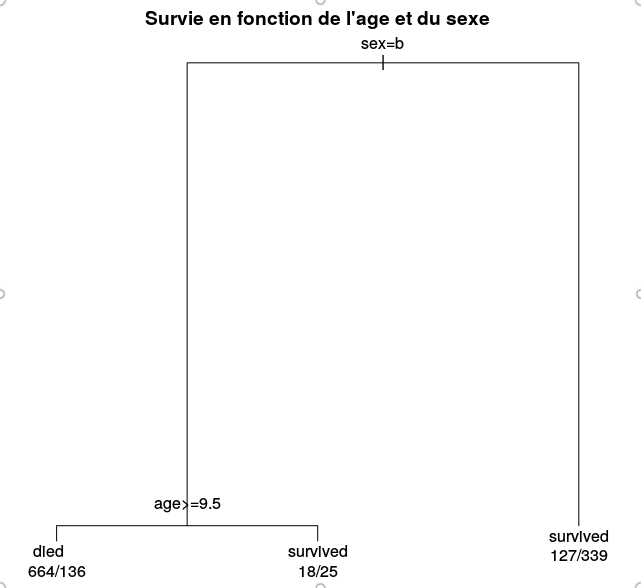
\includegraphics[width=.5\textwidth,height=1\textheight,keepaspectratio]{img/plot.png}%
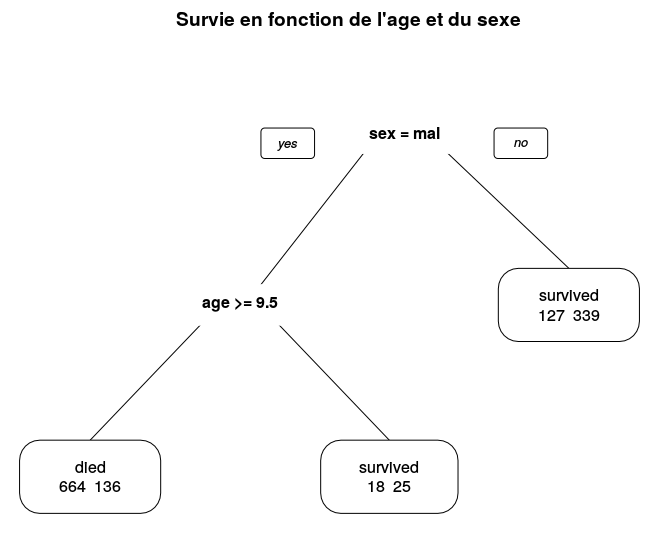
\includegraphics[width=.5\textwidth,height=1\textheight,keepaspectratio]{img/prp.png}
\end{frame}

\begin{frame}
\frametitle{Arbre final}

      \begin{center}
           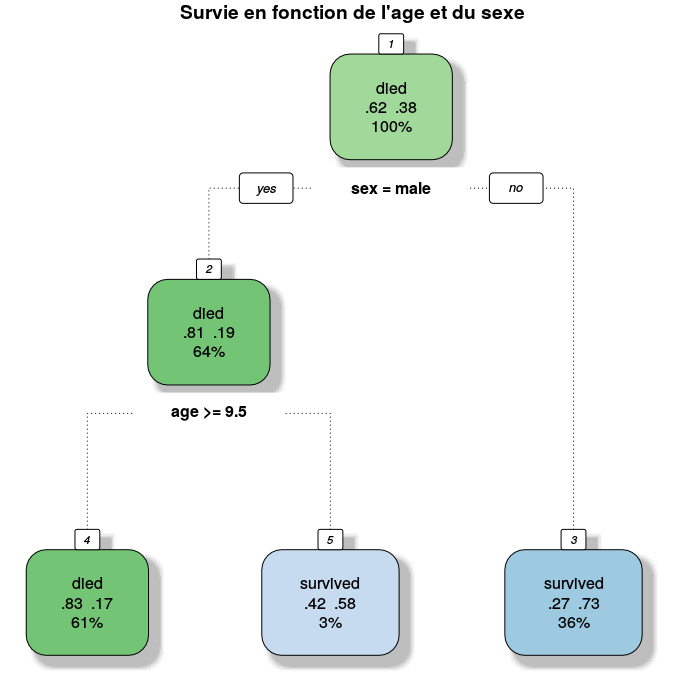
\includegraphics[width=\textwidth,height=0.8\textheight,keepaspectratio]{img/fancy.png}
        \end{center}
\end{frame}

\begin{frame}
\frametitle{Arbre final}
Cet arbre nous donne les informations suivantes : \newline
\begin{itemize}
 \item Le pourcentage de la population totale que contient chaque noeud,
 \item Le pourcentage de personnes mortes et vivantes dans chaque noeud,
 \item La prédiction de la valeur de la variable \textrm{survived} pour chaque noeud,
 \item Les différents test sur les variables.
\end{itemize}

\end{frame}
\begin{frame}
 \frametitle{Vérification du choix des tests}
Nous allons montrer que cet arbre respecte l'algorithme de création décrit précédemment. Pour la survie en fonction de l'age et du sexe, l'arbre va devoir décider quelle
variable prendre en premier pour la séparation. La meilleure variable est celle avec la meilleure valeur de perte d'impureté. \\
Comme calculé précédemment la valeur pour sexe est 0.1319704, nous avons calculés que l'age qui donnera le meilleur résultat de différence d'impureté est \textrm{age = 9.5} et donnera
une valeur de 0.0915799.\newline

Le sexe étant la variable avec la meilleure valeur, elle permettra une meilleure séparation des données. L'arbre respecte bien ce fait en choisissant d'abord la variable sexe pour
classer les données.
\end{frame}

\subsection{Prédiction de la valeur d'une variable}
\begin{frame}
\frametitle{Prédiction de la valeur d'une variable}
L'étape d'apprentissage ayant créé l'arbre via les données d'apprentissage, nous pouvons maintenant tenter de déterminer la valeur de la variable \textrm{survived}
en fonction des autres variables. Pour se faire, il suffit de suivre la branche de l'arbre pour laquelle les variables répondent au tests.\newline
 Nous allons utiliser des personnes pour lesquelles nous connaissons l'age, le sexe, la classe et le nombre de membres de la famille dans le bateau et nous prédirons
 si cette personne a survécu ou non en parcourant l'arbre.\newline

Cette étape se fait via la fonction \textrm{predict}. \newline
 \lstinputlisting{predict.r}
\end{frame}
\begin{frame}
\frametitle{Prédiction de la valeur d'une variable}
 \lstinputlisting{valPredicted.R}

Nous prédisons ainsi le sort des 10 premiers passagers et le comparons aux valeurs théoriques obtenues. Nous remarquons que l'arbre a prédit correctement le sort
de sept des dix passagers.
\end{frame}

\section*{Sources}
\begin{frame}
\frametitle{Sources}
\url{http://apiacoa.org/blog/2014/02/initiation-a-rpart.fr.html}\\
\url{http://www.grappa.univ-lille3.fr/polys/apprentissage/sortie004.html}\\
\url{http://pageperso.lif.univ-mrs.fr/~cecile.capponi/lib/exe/fetch.php?media=cours-arbres.pdf}\\
\url{http://perso.ens-lyon.fr/lise.vaudor/classification-par-arbres-decisionnels/}
\end{frame}

\end{document}